\section{Sindicalismo Europeu}

{
\usebackgroundtemplate{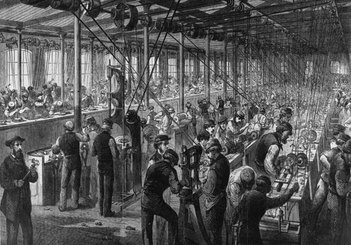
\includegraphics[width=\paperwidth]{Images/english_factory.jpg}}    
\begin{frame}{\colorbox{white}{\textcolor{black}{Sindicalismo Europeu - Conjuntura}}}
    \begin{itemize}
        \colorbox{white}{\textcolor{black}{
        \item Século XVIII:\ fase industrial do capitalismo
        }}
        \colorbox{white}{\textcolor{black}{
        \item Máquinas a vapor x Produção artesanal e manufatureira
        }}
        \colorbox{white}{\textcolor{black}{
        \item Desemprego: exército industrial de reserva
        }}
        \colorbox{white}{\textcolor{black}{
        \item \textbf{\textcolor{red}{Redução dos salários: reprodução da força de trabalho}}
        }}
        \colorbox{white}{\textcolor{black}{
        \item Superexploração: jornada de 18 horas e trabalho infantil
        }}
        \colorbox{white}{\textcolor{black}{
        \item Condições de vida desumanas: residências precárias
        }}
        \colorbox{white}{\textcolor{black}{
        \item Capitalistas organizados x Trabalhadores dispersos
        }}
    \end{itemize}
\end{frame}
}

\begin{frame}{Sindicalismo Europeu - Início}
    Reivindicações
    \begin{itemize}
        \item \textbf{\textcolor{yellow}{Manutenção de um salário digno: sobrevivência}}
        \item Relação (coletiva?) entre patrão e trabalhador
        \item Jornada de trabalho menos extenuante
    \end{itemize}
    Princípios
    \begin{itemize}
        \item Solidariedade e defesa da classe trabalhadora
        \item Revolta contra o capitalismo e a sociedade burguesa
    \end{itemize}
\end{frame}

\begin{frame}{Sindicalismo Europeu - Ludismo}
    \begin{itemize}
        \item 1779: Ned Ludd, operário inglês do Leicestershire
        \item \textbf{\textcolor{yellow}{Primeira manifestação de revolta: destruição das máquinas}}
        \item Outros alvos: matéria-prima, produtos e propriedade privada
        \item Pressão nos empregadores e solidariedade entre os trabalhadores
        \item Situações isoladas: operários condenados pela sociedade
    \end{itemize}
\end{frame}

\begin{frame}{Sindicalismo Europeu - Conquistas iniciais}
    \begin{itemize}
        \item 1824: Parlamento inglês vota a Lei de Livre Associação
        \item Contexto: Associações sindicais violentamente reprimidas
        \item Direito obtido a partir de lutas da classe proletária
        \item \textbf{\textcolor{yellow}{Consequência: trade-unions se desenvolvem pelo país}}
    \end{itemize}
\end{frame}

\begin{frame}{Sindicalismo Europeu - Trade-Unions}
    \begin{itemize}
        \item Salário fixo para toda a categoria
        \item Regulamentação do salário em função do lucro
        \item \textbf{\textcolor{yellow}{Surgimento das greves: caixas de resistência}}
    \end{itemize}
\end{frame}

\begin{frame}{Sindicalismo Europeu - Centralização}
    \begin{itemize}
        \item 1830: Associação Nacional para Proteção do Trabalho
        \item Atuar como central de todos os sindicatos
        \item A Voz do Povo: periódico lançado pelo operariado fabril
        \item \textbf{\textcolor{yellow}{Socialização de informações, negociações e ideias}}
    \end{itemize}
\end{frame}


